\chapter{Desenvolvimento}

Diferente de muitas outras interfaces de desenvolvimento, o KDevelop permite ao usuário incorporar qualquer projeto de software na IDE, contanto que siga alguns padrões já estabelecidos. Boa parte das configurações utilizadas no projeto são oriundas dos gerenciadores de compilação, minimizando o trabalho do usuário.

\section{Ferramentas Utilizadas}
As seguintes ferramentas foram utilizadas para desenvolvimento do projeto.
\begin{itemize}
 \item \textbf{KDevelop}: Editor de código para desenvolvimento do plugin e na realização de debug.
 \item \textbf{QT Framework}: Kit de ferramentas e bibliotecas para desenvolvimento de software.
 \item \textbf{KDE Framework}: Coleção de ferramentas e bibliotecas do KDE.
 \item \textbf{Avrdude}: Programa de carregamento de código para microcontroladores AVR.
 \item \textbf{OpenOCD}: Ferramenta para comunicação de programadores.
 \item \textbf{Placas de desenvolvimento}: Arduino mini, nano, mega, due, uno para testes de suporte utilizando avrdude e Stellaris como EK-LM4F232 para testes utilizando o OpenOCD.
\end{itemize}

O trabalho segue a filosofia GNU \cite{filosofia}, onde, todas as ferramentas utilizadas para o desenvolvimento do plugin são de código aberto e totalmente gratuitas para qualquer um que queira replicar, modificar e contribuir com o projeto.


\subsection{Arduino \textit{toolkit}}
O Arduino \textit{toolkit} possui inúmeras bibliotecas e arquivos de configuração, contendo informações como \textit{bootloader}, configurações de registradores, pinos, funções, entre outros.

O \textit{toolkit} foi utilizado para extração das opções de configuração, podendo dar destaque ao arquivo \textit{boards.txt}.

\lstinputlisting[caption={Parte referente ao Arduino nano de boards.txt},label=boardstxt]{boards.txt}

Dentro deste arquivo se pode extrair várias informações pertinentes para o sistema, como:
\\
\\
\sectionsleft{\textbf{Variáveis de carregamento}}

As configurações para o \textit{bootloader}, hardware de comunicação e processador são:

\begin{itemize}
\item \textit{upload.tool} - Ferramenta para envio do código de máquina.

\item \textit{upload.protocol} - Protocolo de comunicação com o \textit{bootloader}.
%http://www.atmel.com/images/Atmel-8271-8-bit-AVR-Microcontroller-ATmega48A-48PA-88A-88PA-168A-168PA-328-328P_datasheet_Complete.pdf

%http://www.avrfreaks.net/forum/self-programming-and-lock-bits

\item \textit{bootloader.tool} - Ferramenta responsável pela comunicação com o \textit{bootloader}.

\item \textit{bootloader.unlock\_bits} - Bits para desbloquear o \textit{bootloader} na realização de escrita.

\item \textit{bootloader.lock\_bits} - Bits para bloquear o \textit{bootloader} na realização de escrita.

\end{itemize}

As categorias de \textit{upload} possuem as configurações utilizadas para o hardware de comunicação com o \textit{bootloader} e seu protocolo de comunicação.

A categoria de \textit{bootloader} possui as configurações do mesmo assim como as ferramentas utilizadas para sua utilização. As variaveis \textit{unlock\_bits} quanto \textit{lock\_bits} contram o sistema de programação externa de processador, como ISP (\textit{In-Circuit Serial Programmer}), JTAG, entre outros \cite{fuseSettings}. 
\abreviatura{ISP}{\textit{In-Circuit Serial Programmer}}
\\
\\
\textbf{Variáveis de configuração do processador e compilação}

O hardware da placa precisa ser configurado de acordo com as especificações do usuário, o arquivos boards.txt possui as variáveis para as opções de configuração.

\begin{itemize}

\item \textit{build.f\_cpu} - Clock do processador programado, configurado via \textit{bootloader}.

\item \textit{build.board} - Nome da placa.

\item \textit{build.core} - Tipo de hardware.

\item \textit{build.mcu} - Processador utilizado\cite{ATmega48A}.

\item \textit{build.variant} - Topologia do hardware.

\item \textit{upload.maximum\_size} - Espaço livre na \textit{flash}, descontando \textit{bootloader}.

\item \textit{upload.maximum\_data\_size} - Espaço livre na \textit{RAM}.

\item \textit{upload.speed} - Velocidade da comunicação com o \textit{bootloader}.

%http://archive.fabacademy.org/archives/2016/doc/fuses.html
\item \textit{upload.low\_fuses} - Bits menos significativos de configuração do comportamento do hardware.

\item \textit{upload.high\_fuses} - Bits mais significativos de configuração do comportamento do hardware.

\item \textit{upload.extended\_fuses} - Bits estendidos de configuração do comportamento do hardware.

\item \textit{upload.bootloader\_file} - Nome do arquivo que contem o código de máquina do sistema de \textit{bootloader}.

\end{itemize}

As categorias \textit{build} são configurações para o processo de compilação, especificando o processador, tipo de placa e clock. A categoria upload é responsável pelas limitações do tamanho do código de maquina da aplicação, sua velocidade de transmissão para o processador, o local do código de maquina do \textit{bootloader} e as configurações de programação do processador, realizada pelos \textit{fuses}. 

Os Bytes com memória não volátil do processador, conhecidos como \textit{low\_fuses}, \textit{high\_fuses} e \textit{extended\_fuses}, tem como responsabilidade determinar o comportamento do processador. Estes podem controlar o consumo energético, geração de clock, tempo de boot, tipo de clock, pino de reinicialização, modo de depuração, modo de programação, falhas de operação, monitor da tensão de alimentação, entre outros\cite{fuseSettings}\cite{fuses}.
\\
\\
\textbf{AVRDUDE}

Ferramenta responsável para programar maioria das placas da Arduino, possui várias opções necessárias para programar o sistema embarcado, dentro destas, pode-se destacar.

\begin{itemize}
\item \textit{partno} - Processador utilizado.

\item \textit{baudrate} - Velocidade de comunicação com o \textit{bootloader}.

\item \textit{config-file} - Arquivo de configuração do processador.

\item \textit{programmer} - Hardware utilizado para realizar o processo de gravação.

\item \textit{port} - Porta de comunicação com o hardware.

\item \textit{memtype} - Configuração da memória do processador.

\item \textit{filename} - Arquivo que contem o código de máquina.

\item \textit{U} - Além do \textit{memtype} e \textit{filename}, é possível passar o parâmetro \textit{U} junto com configurações de \textit{fuses} e \textit{lock/unlock} bits.
\end{itemize}

Para utilizar essas configurações é necessário um conhecimento do funcionamento do hardware e como essas opções afetam o sistema embarcado. 

\subsection{OpenOCD}

Recebe como argumentos os parâmetros de configuração ou comandos para a comunicação do JTAG. As opções disponíveis são:

\begin{itemize}
\item {file} - Aponta o arquivo de configuração.
\item {debug} - Nível da mensagem de depuração.
\item {command} - Executa um comando do OpenOCD.
\end{itemize}

Um exemplo de comando utilizado com a ferramenta, pode ser visto no Algoritmo \ref{openocdcli}, \ref{lm4f232cfg} e \ref{tiicdicfg}.

\lstinputlisting[caption={Linha de comando do OpenOCD},label=openocdcli]{openocdcli.txt}

%%/usr/share/openocd/scripts/board/ek-lm4f232.cfg
\lstinputlisting[caption={board/ek-lm4f232.cfg},label=lm4f232cfg]{ek-lm4f232.cfg}

%/usr/share/openocd/scripts/interface/ti-icdi.cfg
\lstinputlisting[caption={interface/ti-icdi.cfg},label=tiicdicfg]{ti-icdi.cfg}

%/usr/share/openocd/scripts/target/stellaris.cfg

Onde \$\{bin\} é definido pelo caminho do arquivo de código de máquina e os valores de PID e VID pelo \textit{usbutils}.
Para criar o arquivo de configuração do OpenOCD, é necessário o conhecimento das características e do funcionamento do hardware.

\section{Fluxo de trabalho}

A interface de projeto existente no KDevelop permite que boa parte das especificações de projeto fiquem no sistema de geração automatizada\footnote{Entre eles pode se destacar os mais utilizados são o \textit{Makefile}, \textit{CMakefile} e \textit{WAF}.}, permitindo o desenvolvimento de software sem a integração do projeto com o KDevelop para sua utilização.
\iffalse
, utilizando arquivos intermediários de configuração\footnote{Arquivos que contem informações sobre compilador, estilo de código, execução e etc.}.
\fi
Esta flexibilidade de integração de projetos no KDevelop acrescenta um grau de dificuldade na realização do plugin, pois, as informações necessárias no carregamento do binário para o sistema embarcado necessita de sua localização e da porta de comunicação para o hardware em desenvolvimento. %\itodo{ADICIONAR MAIS INFORMAÇÕES DE FLUXO}

\section{Desenvolvimento do software}

\begin{figure}[!htb]
  \centering
  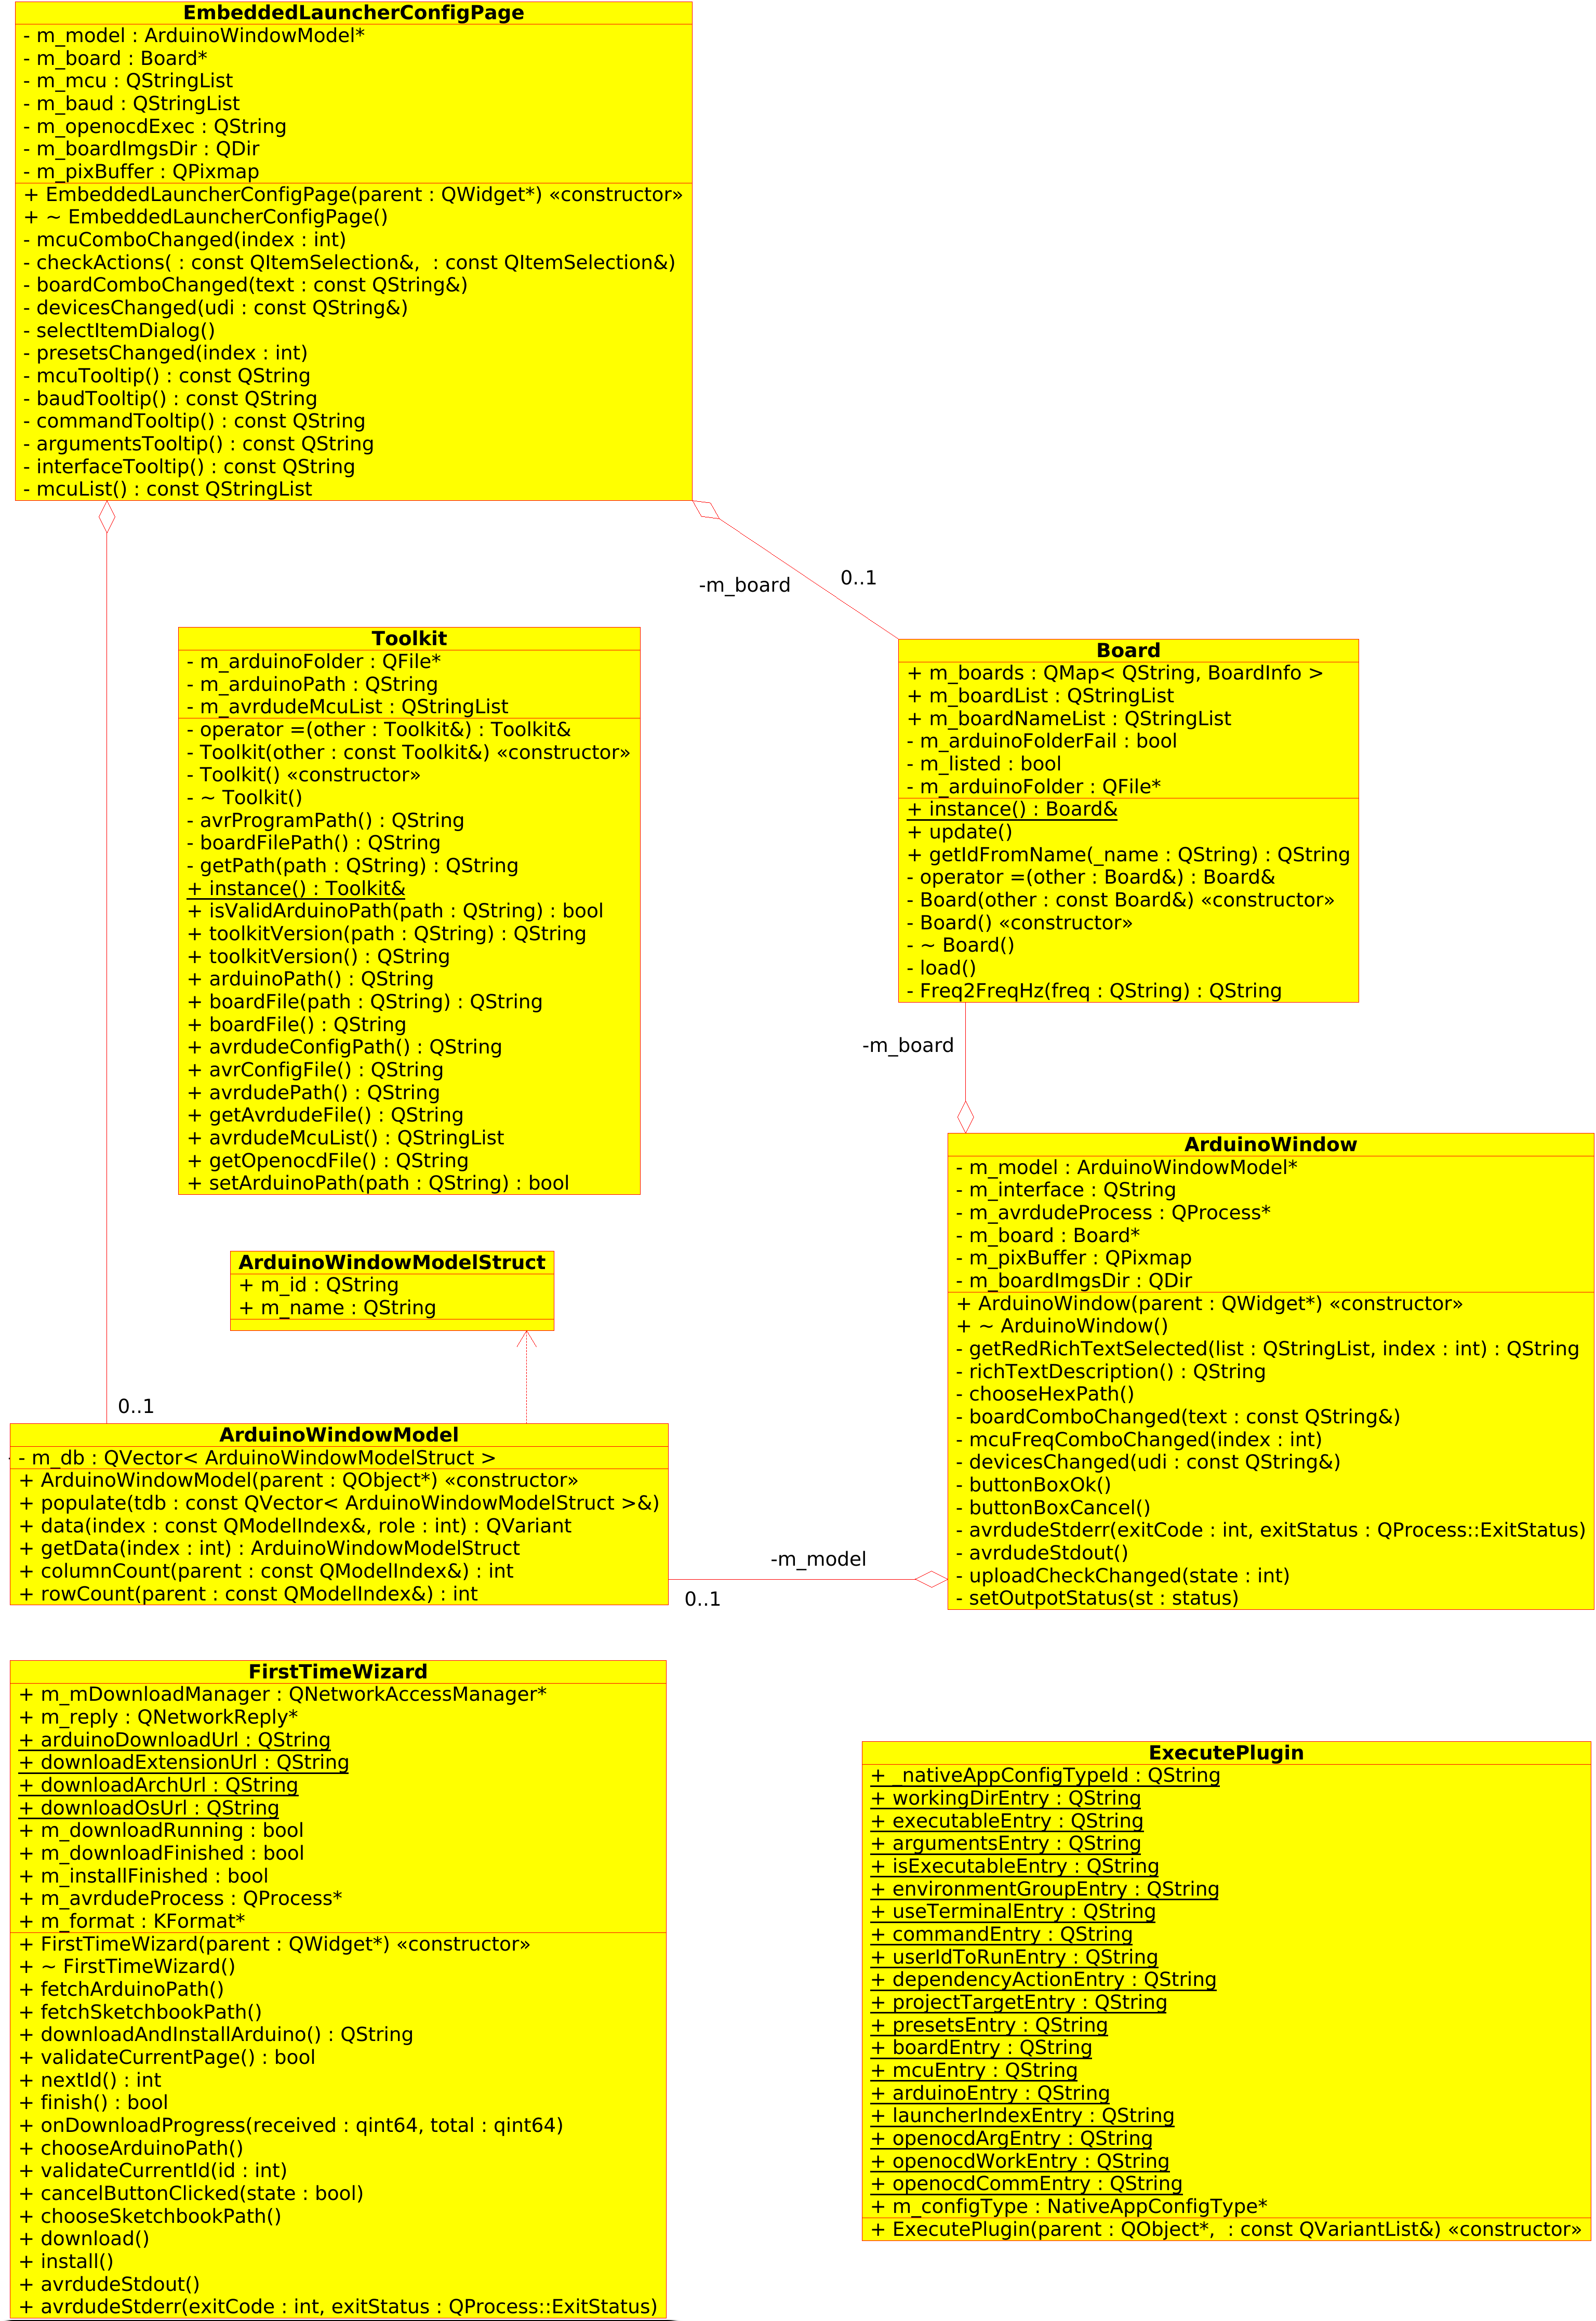
\includegraphics[width=0.85\textwidth]{figuras/uml.png}
  \caption[UML proposto]{UML proposto para desenvolvimento do plugin.}
  \label{fig:uml}
\end{figure}

\abreviatura{UML}{Unified Modeling Language}

O plugin (\figref{fig:uml}) foi integrado no KDevelop (\figref{fig:kdevelop}) via a utilização de ferramentas básicas de desenvolvimento para o mesmo (\textit{kdevplatform}). Nesta seção, será demonstrando as interfaces desenvolvidas e sua integração com o KDevelop.

\begin{figure}[!htb]
  \centering
  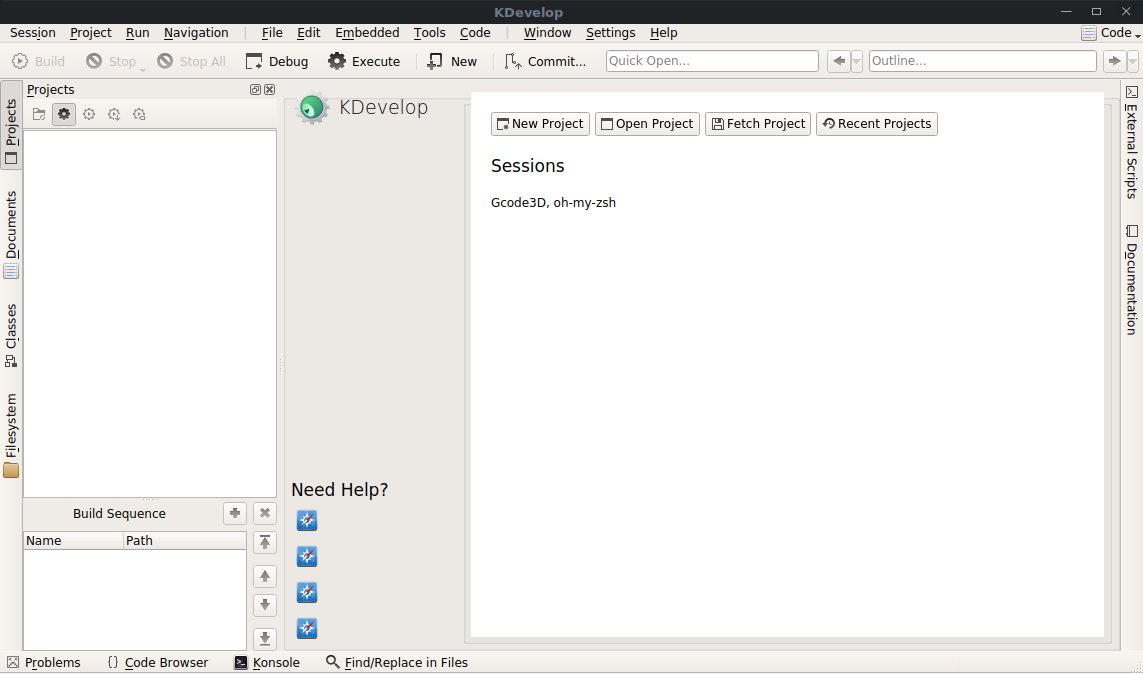
\includegraphics[width=0.85\textwidth]{figuras/kdevelop.png}
    \caption[KDevelop]{KDevelop.}
    \label{fig:kdevelop}
\end{figure}

\subsection{Menu de acesso}

O menu de acesso (\figref{fig:kdevelopMenu}), foi desenvolvido para realizar duas funções, configurar o plugin em relação as ferramentas necessárias para sua utilização com as placas da \textit{Arduino} (\textit{Arduino Setup}), e permitir a realização do carregamento de código desenvolvido para a placa, utilizando uma interface gráfica assistencialista (\textit{Board settings}).

\begin{figure}[!htb]
  \centering
  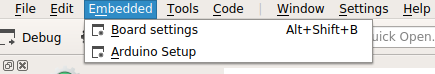
\includegraphics[width=0.95\textwidth]{figuras/kdevelopMenu.png}
  \caption[Menu do plugin no KDevelop]{Menu de acesso do plugin no KDevelop.}
  \label{fig:kdevelopMenu}
\end{figure}

\subsection{Arduino Setup}

Realiza a configuração inicial do plugin no sistema, permitindo ao usuário escolher uma versão do kit de ferramenta do \textit{Arduino} para utilizar ou a instalação automática do kit pelo plugin.

Primeiramente foi definido um diagrama inicial de estados para facilitar a compreensão da configuração (\figref{fig:ftwstate}).

\begin{itemize}
\item \textbf{\textit{First-Time Configuration} (FTC)}: Tela inicial, permitindo ao usuário escolher o local do \textit{toolkit} previamente instalado (\figref{fig:kdevelopinstaller1}), ou escolher a opção de instalação automática. 

\item \textbf{\textit{Automatic Instalation} (AutoInst)}: Tela resultante da escolha da instalação automática na configuração inicial do \textbf{\textit{First-Time Configuration}}. Essa, separada em duas etapas, \textit{Download} e \textit{Install}.

\subitem \textbf{\textit{Download} (Down)}: É realizado a comunicação com o servidor oficial resultando no download das ferramentas necessárias (\figref{fig:kdevelopinstaller21}).

\subitem \textbf{Install}: Após o \textit{download} é realizado a decomposição e instalação do conjunto de ferramentas (\figref{fig:kdevelopinstaller22}).

\item \textbf{\textit{End Configuration} (EndConf)}: Tela final, resulta após a escolha de um \textit{toolkit} previamente instalado ou após a conclusão da instalação automática (\figref{fig:kdevelopinstaller3}).
\end{itemize}

\begin{figure}[htb!]
  \centering
  \begin{tikzpicture}[->,>=stealth',shorten >=1pt,auto,node distance=2.8cm,semithick]
    \tikzstyle{every state}=[fill=blue,draw=none,text=white]

	%First-Time Configuration
    \node[state]         (A)                    {$FirstTimeConf.$}; 
    % Automactic Install
    \node[state]         (B) [right of=A]       {$Auto Inst.$};
    \node[state]         (C) [right of=B]       {$Down.$};
    \node[state]         (D) [below of=C]       {$Install$};
    \node[state]         (E) [below of=A]       {$EndConf$};

    \path (A) edge              node {Existing Installation}      (E)
	      (A) edge  [bend left]   node {Automatic Installation}      (B)
          (B) edge              node {}      (C)
          (C) edge              node {}      (D)
          (D) edge              node {}      (E);
  \end{tikzpicture}
  \caption[Diagrama de estados do \textit{First-Time Wizard}]{Diagrama de estados do \textit{First-Time Wizard}}
  {\label{fig:ftwstate}}
\end{figure}


\begin{figure}[!htb]
  \centering
  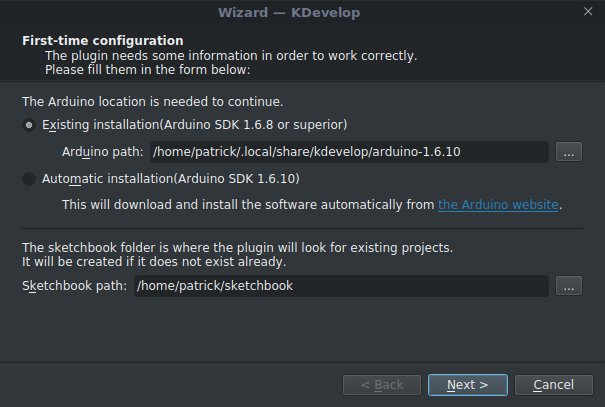
\includegraphics[width=0.85\textwidth]{figuras/kdevelopInstaller1.png}
  \caption[Fist-Time Configuration]{\textit{Fist-Time Configuration} com \textit{Existing Installation} selecionado.}
  \label{fig:kdevelopinstaller1}
\end{figure}

\begin{figure}[!htb]
  \centering
  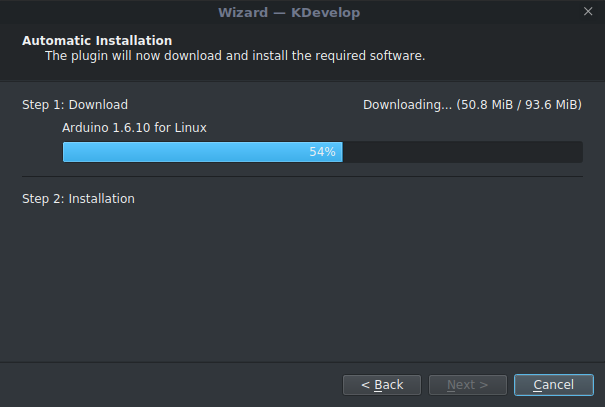
\includegraphics[width=0.85\textwidth]{figuras/kdevelopInstaller21.png}
  \caption[Automatic Instalation executando Download]{\textit{Automatic Instalation} com \textit{download} em andamento.}
  \label{fig:kdevelopinstaller21}
\end{figure}

\begin{figure}[!htb]
  \centering
  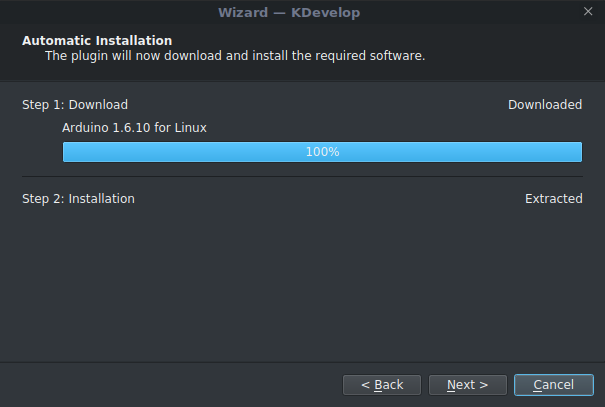
\includegraphics[width=0.85\textwidth]{figuras/kdevelopInstaller22.png}
  \caption[Automatic Instalation pós instalação]{Automatic Instalation após a instalação do \textit{toolkit}.}
  \label{fig:kdevelopinstaller22}
\end{figure}

\begin{figure}[!htb]
  \centering
  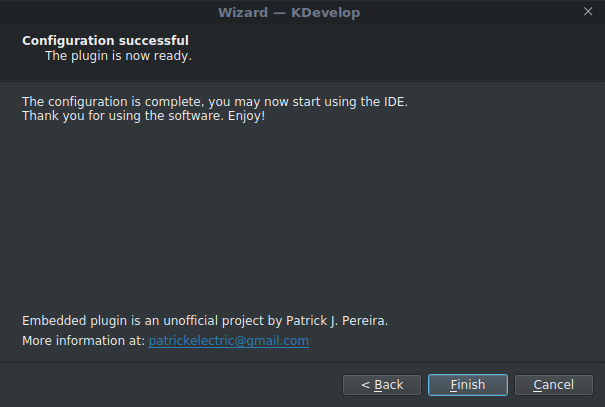
\includegraphics[width=0.85\textwidth]{figuras/kdevelopInstaller3.png}
  \caption[End Configuration]{End Configuration}
  \label{fig:kdevelopinstaller3}
\end{figure}

\subsection{Board Settings}

Interface para realizar o envio do binário para o sistema embarcado, permitindo o usuário interagir com o sistema, escolhendo a placa e algumas opções simples como processador, frequência, interface de comunicação, tipo de log de dados da saída do \textit{bootloader}. Além de permitir visualizar e mostrar quais opções foram selecionadas (\figref{fig:boardsettings}).

\begin{figure}[!htb]
  \centering
  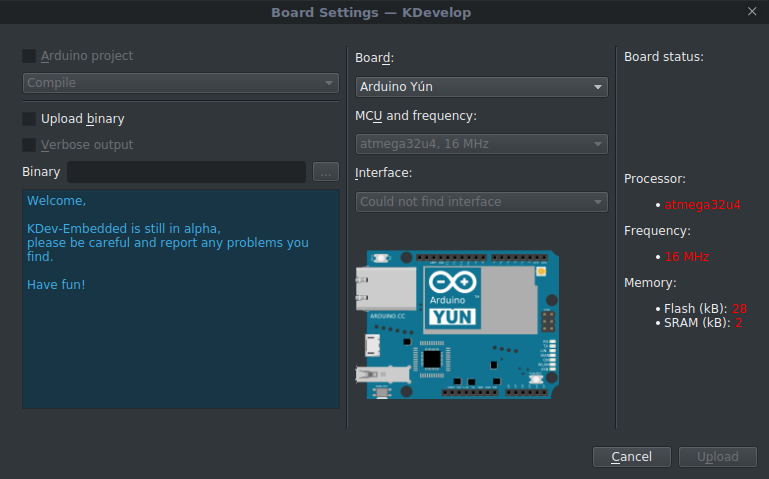
\includegraphics[width=0.85\textwidth]{figuras/boardsettings.png}
  \caption[Board Settings com configuração inicial]{\textbf{Board Settings} sem configuração prévia.}
  \label{fig:boardsettings}
\end{figure}

Após ter o acesso a interface, o usuário pode escolher a opção de \textit{Upload Binary}, selecionando desta forma um arquivo contendo o código de máquina (\textit{Blink.hex}), após isso, pode-se escolher no menu \textit{Board} a placa para programar, permitindo ao plugin selecionar as opções para o hardware indicado, além disso, é necessário selecionar o tipo de processador e clock, como consta no menu \textit{MCU and frequency}, tendo isto selecionado, a ultima configuração necessária para realizar o envio do código é a porta que consta no menu \textit{interface}. Essas configurações podem ser visualizadas na \figref{fig:boardsettingsserial}, onde foi escolhido um Arduino Nano contendo um processador atmega328p com um clock de $16MHz$ utilizando uma interface de programação \textit{FT232 USB UART}.

\begin{figure}[!htb]
  \centering
  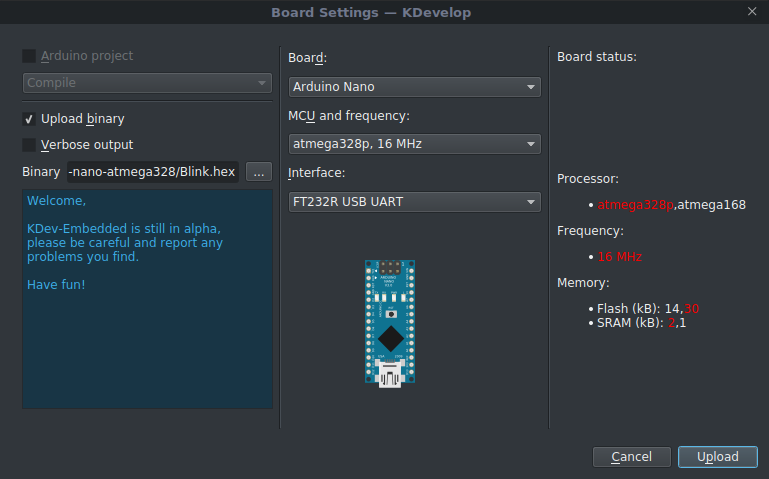
\includegraphics[width=0.85\textwidth]{figuras/boardsettingsSerial.png}
  \caption[Board Settings após configuração para envio]{\textbf{Board Settings} após configuração do usuário.}
  \label{fig:boardsettingsserial}
\end{figure}

Depois de tudo configurado, é possível clicar no botão \textit{upload} e realizar o envio do binário selecionado para placa. Podendo acarretar no sucesso da operação (\figref{fig:boardsettingsdone}) ou na sua falha (\figref{fig:boardsettingsndone}).

\begin{figure}[!htb]
  \centering
  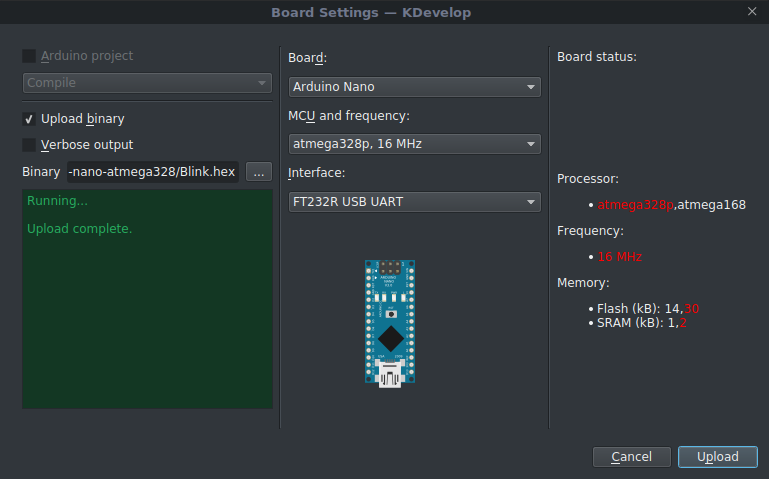
\includegraphics[width=0.85\textwidth]{figuras/boardsettingsdone.png}
  \caption[Board Settings com sucesso no envio]{\textbf{Board Settings} após o envio do código para o sistema embarcado.}
  \label{fig:boardsettingsdone}
\end{figure}

\begin{figure}[!htb]
  \centering
  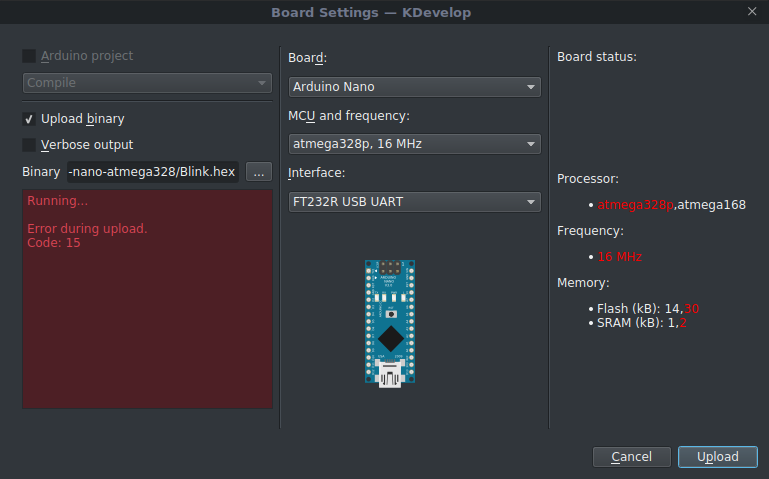
\includegraphics[width=0.85\textwidth]{figuras/boardsettingsndone.png}
  \caption[Board Settings com falha no envio]{Imagem do \textbf{Board Settings} após falha no envio do código para o sistema embarcado.}
  \label{fig:boardsettingsndone}
\end{figure}

\section{Integração com fluxo de trabalho}
Além do desenvolvimento do software, permitindo seu uso como projetado inicialmente, foi necessário reservar uma parte do período do projeto para modificações de interface gráfica e de organização de layout, permitindo um uso simplificando para usuários não tão avançados, e ao mesmo tempo uma flexibilidade aos usuários com conhecimento profundo do funcionamento do sistema, modificando e personalizando as opções fornecidas pelo ambiente gráfico, sem restringir o alto nível de abstração que essas ferramentas já permitem.

\subsection{Integração e compilação do projeto}

Para o usuário realizar a compilação, é necessário importar um projeto: Project $\rightarrow$ Open / Import Project... e importar um projeto com um sistema de compilação suportado pelo KDevelop, seguindo o fluxo de trabalho do KDevelop (\figref{fig:importproject}).

\begin{figure}[!htb]
  \centering
  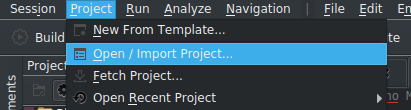
\includegraphics[width=1\textwidth]{figuras/importproject.png}
  \caption[Import Project]{Import Project.}
  \label{fig:importproject}
\end{figure}

Após o projeto ser importado com sucesso, será possível visualizar o mesmo no menu de projeto (\figref{fig:projects}).

\begin{figure}[!htb]
  \begin{minipage}[t]{0.5\textwidth}
  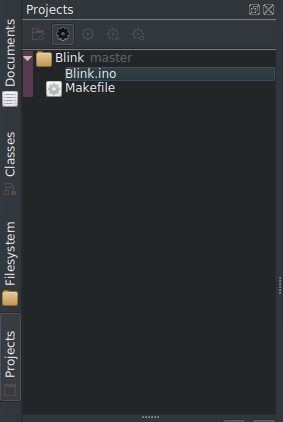
\includegraphics[width=0.7\textwidth]{figuras/projects.png}
  \caption[Projects antes da compilação]{Dock Projects antes\\ da compilação do projeto.}
  \label{fig:projects}
  \end{minipage}%
  \begin{minipage}[t]{0.5\textwidth}
%  \raggedleft
  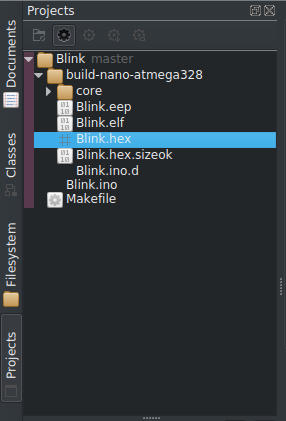
\includegraphics[width=0.713\linewidth]{figuras/projects2.png}
  \caption[Projects depois da compilação]{Dock Projects depois\\ da compilação do projeto.}
  \label{fig:projects2}
  \end{minipage}
\end{figure}

Depois de ter realizado a importação com sucesso, é necessário realizar a compilação para gerar o binário que será enviado para o processador, realizando o processo de compilação, basta clicar no botão \textit{Build} da interface do KDevelop, após isso, o menu de projeto se atualizado, podendo ser possível visualizar o arquivo com o código de máquina (\figref{fig:projects2}).

\subsection{Lançamento}

Seguindo o fluxo de trabalho do KDevelop, é necessário configurar o projeto para ser realizado o lançamento de uma forma correta. Para tal, basta executar Run $\rightarrow$ Configure Launchs (\figref{fig:run}).

\begin{figure}[!htb]
  \centering
  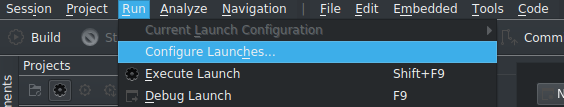
\includegraphics[width=1\textwidth]{figuras/run.png}
  \caption[Configure Launchs]{Configure Launchs.}
  \label{fig:run}
\end{figure}

Após isso, uma tela de configuração será aberta, podendo ser configurado da seguinte forma para um sistema embarcado, Add New... $\rightarrow$ Embedded e modificando o sistema de acordo com o alvo que será programado, \figref{fig:run2}. Nesta, foi utilizado um \textit{Arduino Nano} para realizar o teste de envio de código, também é possível selecionar a opção de \textit{OpenOCD} desenvolvido (\figref{fig:openocd}).

\begin{figure}[!htb]
  \centering
  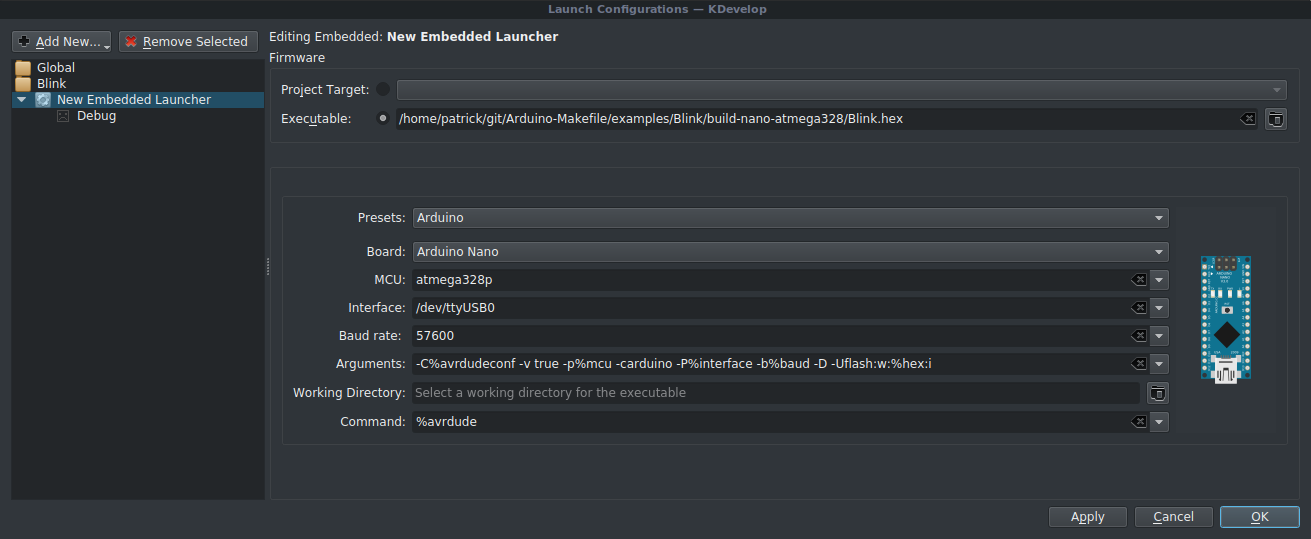
\includegraphics[width=1\textwidth]{figuras/run2.png}
  \caption[\textit{Configure Launchs} para \textit{avrdude}]{Configure Launchs para \textit{avrdude}.}
  \label{fig:run2}
\end{figure}

\begin{figure}[!htb]
  \centering
  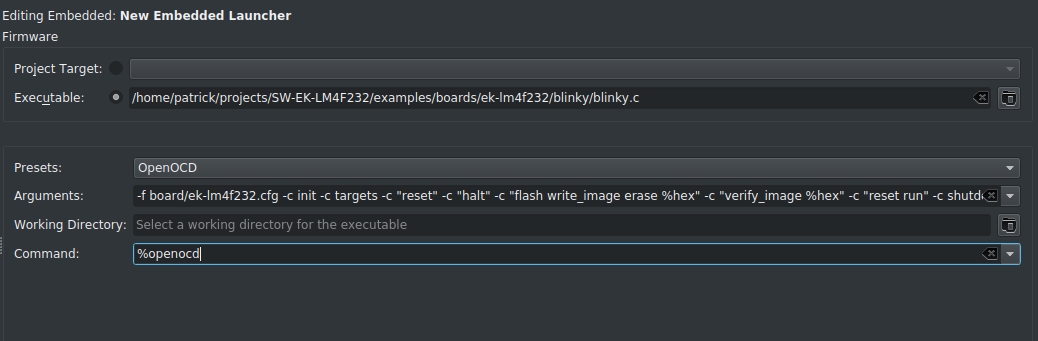
\includegraphics[width=1\textwidth]{figuras/openocd.png}
  \caption[\textit{Configure Launchs} para \textit{OpenOCD}]{Configure Launchs para \textit{OpenOCD}.}
  \label{fig:openocd}
\end{figure}

Após realizar as configurações, basta aplica-las e em seguida executar o lançamento com o botão Execute. Tendo isso realizado, será aberto um console onde todos os dados de gravação serão mostrados (\figref{fig:runavrdude} e \figref{fig:runopenocd}).

Com as configurações salvas no lançador do código, as mesmas ficam reservadas em um arquivo conhecido como *.kdev4, responsável por gerenciar os arquivos de configuração, permitindo que os próximos lançamento sempre utilizem as mesmas configurações, além de permitir outras configurações de lançamento em paralelo.

\begin{figure}[!htb]
  \centering
  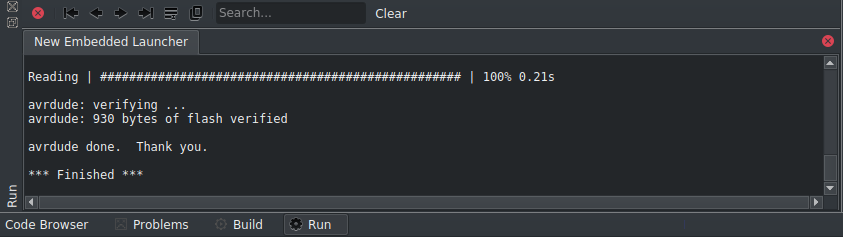
\includegraphics[width=1\textwidth]{figuras/runavrdude.png}
  \caption[\textit{Embedded Launcher} com \textit{avrdude}]{Embedded Launcher com saída do \textit{avrdude.}}
  \label{fig:runavrdude}
\end{figure}

\begin{figure}[!htb]
  \centering
  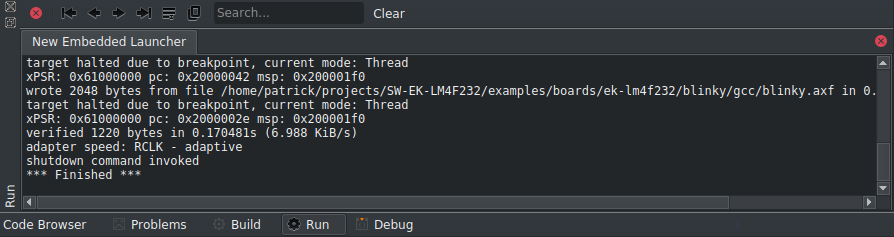
\includegraphics[width=1\textwidth]{figuras/runopenocd.png}
  \caption[\textit{Embedded Launcher} com \textit{openocd}]{Embedded Launcher com saída do \textit{openocd.}}
  \label{fig:runopenocd}
\end{figure}

\subsection{Depuração}

A depuração pode ser realizada utilizando as próprias ferramentas do KDevelop, permitindo uma conexão com o servidor do GDB pela porta padrão, tal configuração foi testada utilizando a implementação do \textit{OpenOCD} (\figref{fig:openocddebug}).

\begin{figure}[!htb]
  \centering
  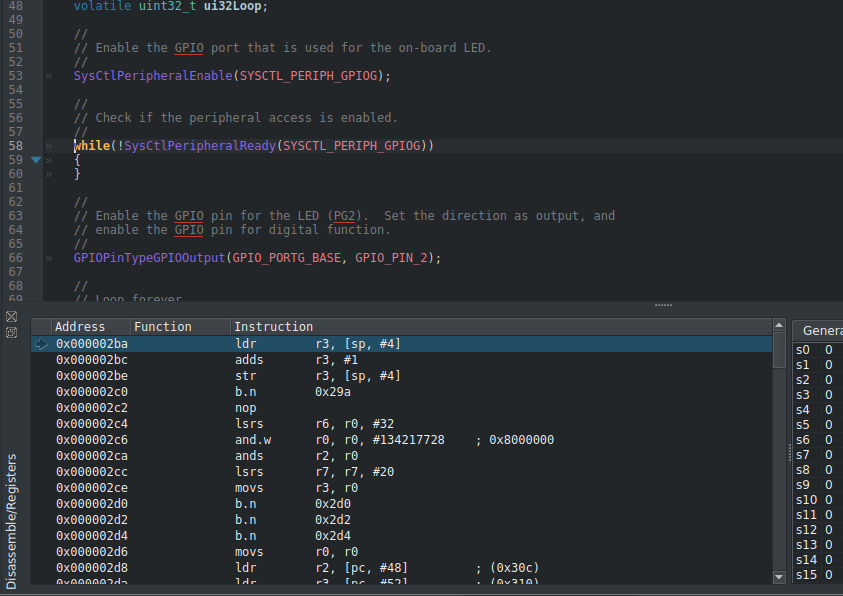
\includegraphics[width=0.85\textwidth]{figuras/DEBUG.png}
  \caption[\textit{Debug mode} com \textit{openocd} no KDevelop]{\textit{Debug mode} com \textit{openocd.} no KDevelop}
  \label{fig:openocddebug}
\end{figure}
